\textbf{ABCD}

\textbf{1. Ma trận ABCD cho hệ quang đồng trục}

Quang hệ đồng trục là một quang hệ bao gồm các quang cụ (lưỡng chất, thấu kính, gương cầu,...) được đặt đồng trục với nhau. Một tia sáng tại một vị trí xác định trong hệ quang đồng trục có thể được mô tả thông qua 2 thông số tọa độ, đó là góc \(\alpha\) mà tia sáng đó hợp với quang trục và khoảng cách \(y\) từ điểm cắt của tia sáng với mặt phẳng xác định vị trí đến quang trục. 

\ \ 

Với mỗi đoạn di chuyển hoặc thay đổi quỹ đạo của tia sáng trong hệ quang đồng trục, ta có thể biểu diễn sự biến đổi tọa độ thông qua 4 tham số \(A\), \(B\), \(C\), \(D\) sao cho thông số tia sáng trước và sau bước biến đổi tuân theo biểu thức:
\begin{align*}
    y' &= A y + B \alpha , \\
    \alpha' &= C y + D \alpha .
\end{align*}

Bộ 4 tham số trên được gọi là "ma trận ABCD".

\begin{figure}[!h]
    \centering
    \begin{subfigure}{0.48\textwidth}
        \centering
        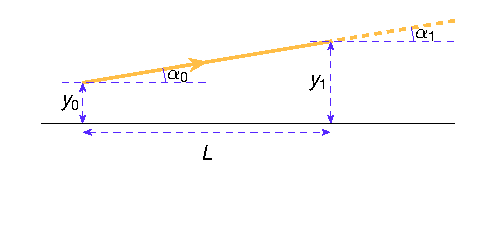
\includegraphics[width=0.9\textwidth]{Problem_4/Figs_P4/Straight_light_ABCD.pdf}
        \caption{Sự thay đổi bộ thông số \( (y, \alpha) \) của tia sáng thẳng.}
        \label{fig:Straight_light_ABCD}
    \end{subfigure}
    \hspace{0.01\textwidth}
    \begin{subfigure}{0.48\textwidth}
        \centering
        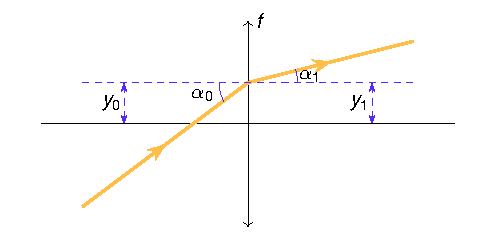
\includegraphics[width=0.95\textwidth]{Problem_4/Figs_P4/Lens_ABCD.pdf}
        \caption{Sự thay đổi bộ thông số \( (y, \alpha) \) của thấu kính hội tụ.}
        \label{fig:Lens_ABCD}
    \end{subfigure}
    \caption{Biến đổi thông số \( (y, \alpha) \) qua các cấu trúc quang học.}
\end{figure}

\textbf{Câu hỏi a. Ma trận biến đổi thẳng}

Xét một tia sáng đi thẳng trong môi trường đồng tính đẳng hướng (Như hình \ref{fig:Straight_light_ABCD}). Hãy tìm bộ ma trận ABCD đối với một đoạn biến đổi ứng với việc tia sáng đi được một khoảng cách \(L\) theo quang trục của hệ.

\ \ 

\textbf{Câu hỏi b. Ma trận thấu kính mỏng}

Một tia sáng gặp một thấu kính hội tụ mỏng với góc tới \(\alpha_0\) và tại vị trí cách quang tâm của thấu kính một khoảng \(y_0\) (như hình \ref{fig:Lens_ABCD}). Tìm ma trận ABCD đối với sự bẻ hướng tia sáng của thấu kính này theo tiêu cự \(f\) của nó.

\ \ 

\textbf{2. Hệ thấu kính, hội tụ và phân kỳ}

Ghép đan xen một hệ các thấu kính hội tụ có tiêu cự \(f_1\) và thấu kính phân kỳ có tiêu cự \(-f_2\) thành một hệ thấu kính vô hạn tuần hoàn (như hình \ref{fig:Infinites_lens}). Khoảng cách từ thấu kính hội tụ trước đến thấu kính sau là \(L_1\) và khoảng cách từ thấu kính phân kỳ trước đến thấu kính hội tụ sau là \(L_2\). 
\begin{figure}[!h]
    \centering
    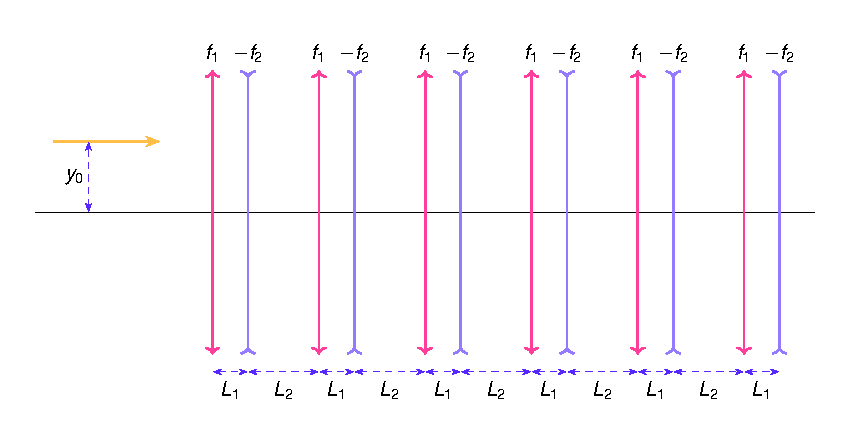
\includegraphics[width=0.9\textwidth]{Problem_4/Figs_P4/Infinite_lens.pdf}
    \caption{Hệ vô hạn thấu kính ghép đan xen.}
    \label{fig:Infinites_lens}
\end{figure}

\ \ 

\textbf{Câu hỏi c.} Tìm ma trận ABCD của một mắt trong mạng thấu kính tuần hoàn bao gồm một thấu kính hội tụ và 1 thấu kính phân kỳ, tính từ điểm bắt đầu mắt là điểm tia sáng gặp thấu kính hội tụ của mắt và kết thúc mắt là điểm tia sáng gặp thấu kính hội tụ ở mắt tiếp theo.

\ \ 

\textbf{Câu hỏi d.} Tìm điều kiện của \(L_1\) và \(L_2\) để tia sáng di chuyển qua vô số thấu kính trong hệ có xu hướng hội tụ về phía quang trục.

\ \ 

\textbf{Câu hỏi e.} Xét một tia sáng tới hệ thấu kính theo phương song song quang trục và cách quang trục một khoảng \(y_0\). Tìm giá trị \(y_n\) và \(\alpha_n\) khi tia sáng vừa ló ra khỏi thấu kính hội tụ thứ \(n\).